\documentclass[a4paper]{article}



%% Sets page size and margins
\usepackage[a4paper,top=2cm,bottom=2cm,left=3cm,right=3cm,marginparwidth=1.75cm]{geometry}

%% Useful packages
\usepackage{amsmath,amsthm,amssymb,amsfonts,graphicx, fancyvrb}
\usepackage{drawstack}

\title{\vspace{-1.5cm}IERG4130 Lab 1 Report}

\author{LAU Long Ching\\SID: 1155127347\\
        
}

\date{13/02/2021}



\begin{document}
\maketitle
\section{Set-UID Program and Linux Capability}
\subsection{Task 1: Environment Variable and Set-UID Programs}
\subsubsection{Step 1-2}
I compiled the above program, change its ownership to root, and make it a Set-UID program.\\\\
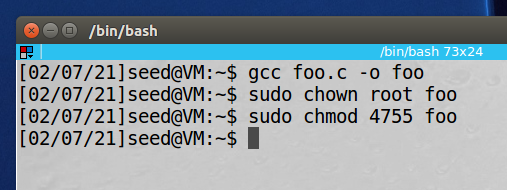
\includegraphics[scale=0.7]{1/1.png}
\subsubsection{Step 3}
Next, I tried to set the following environment variables with the \verb+export+ command. We can see that the child process inherits the \verb+PATH+ and \verb+MY ENV+ environment variable, but there is no \verb+LD+ environment variable as seen in the screenshot. This shows that the SET-UID program's child process may not inherit all the environment variables of the parent process. This is a security mechanism implemented by the dynamic linker. Since the real user id is different from the effective user id, only the other two environment variables are seen in the output.\\\\
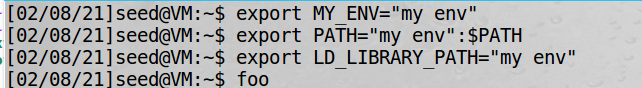
\includegraphics[scale=0.7]{1/2.png}\\\\
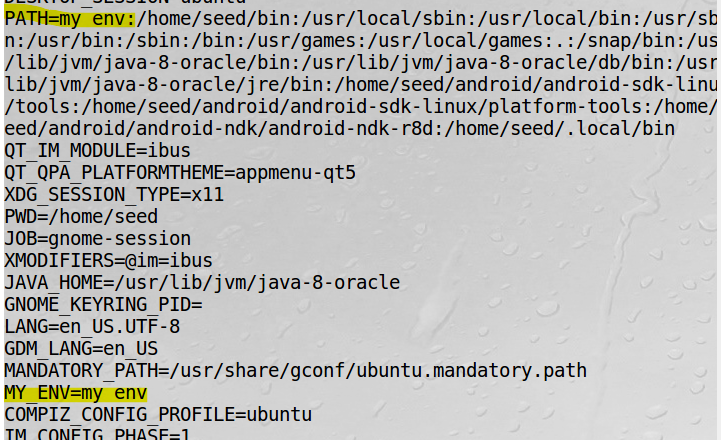
\includegraphics[scale=0.7]{1/3.png}\\
\pagebreak
\subsection{Task 2: Experiencing Capabilities}
\subsubsection{Step 1}
As a normal user, the \verb+ping+ command ran successfully. The probes were well received by the server and were echoed back.\\\\
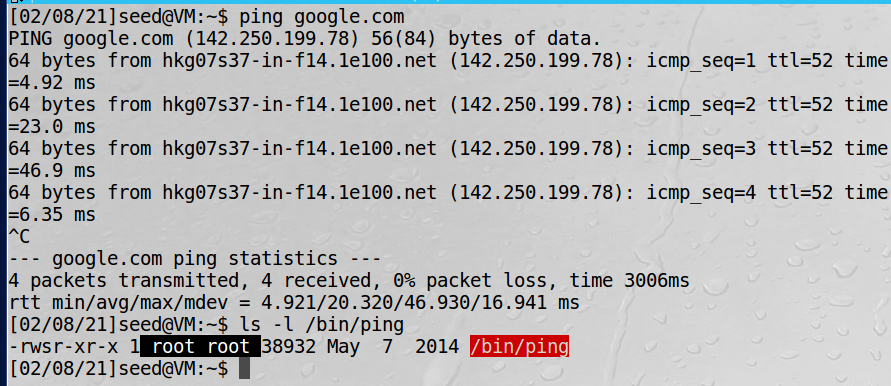
\includegraphics[scale=0.7]{1/6.png}\\\\
Next, we remove the privilege from \verb+ping+ and turn it to a non-Set-UID program. It no longer has root as the effective user id and the command does not work anymore. No RAW sockets were opened.\\\\
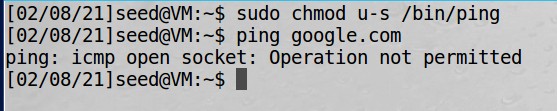
\includegraphics[scale=0.7]{1/7.png}
\subsubsection{Step 2}
I then only assign the \verb+cap_net_raw+ capabilities to ping and use \verb+getcap+ to display the capabilities. It shows that \verb+ping+ now indeed has the capability to send RAW sockets, and the command works again!!\\\\
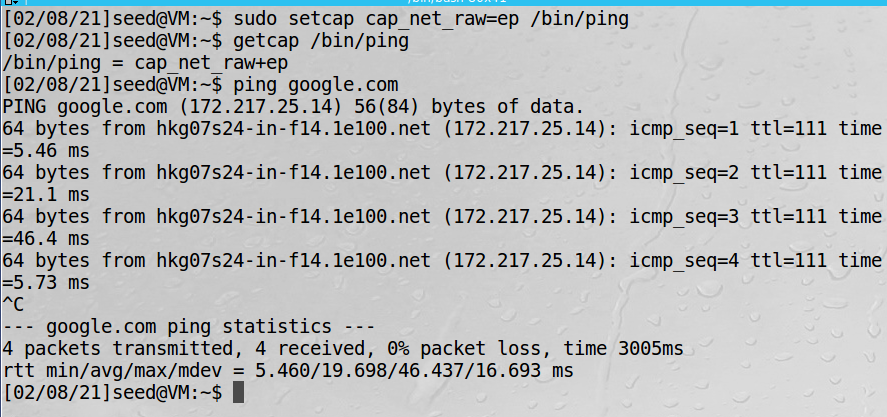
\includegraphics[scale=0.7]{1/8.png}
\subsubsection{Step 3}
Lastly we remove the capabilities with \verb+setcap -r+. Since it does not have the capabilities anymore and it is a non-Set-UID program, the program does not work.\\\\
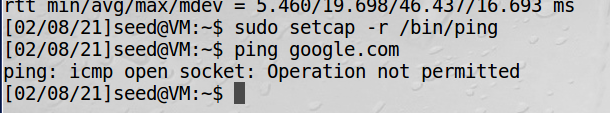
\includegraphics[scale=0.7]{1/9.png}\\
\pagebreak
\section{Buffer-Overflow Vulnerability}
\subsection{Task 3: Running Shellcode}
\subsubsection{Turning off Countermeasures}
I turned off the ASLR and replaced \verb+/bin/sh+ with the shell program \verb+zsh+ provided by SEED LAB.\\\\
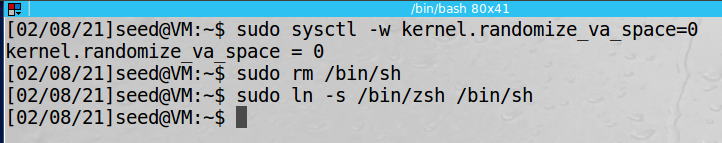
\includegraphics[scale=0.7]{2/1.png}
\subsubsection{Running shellcode}
The assembly version of the above program invoked a shell. It is now ready for the attack.\\\\
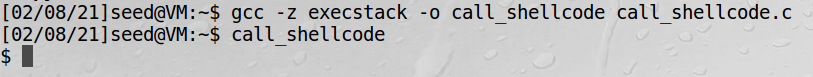
\includegraphics[scale=0.7]{2/2.png}\\\\
Next I compiled the vulnerable program with countermeasures removed, and escalated its privilege.\\\\
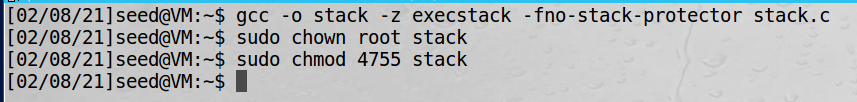
\includegraphics[scale=0.7]{2/3.png}
\subsection{Task 4: Exploiting the Vulnerability}
Now, we are almost ready! for the exploit code \verb+exploit.c+, what we need are the contents we fill the buffer with. I checked the \verb+stack+ program with \verb+gdb+, set a break point at function \verb+bop+. Now we know the address of \verb+ebp+ and \verb+buffer+. Since \verb+0xbfffeb48 - 0xbfffeabe = 138+ and the return address is \verb-ebp+4-, the fake address should begin at \verb-buffer[138+4]-. The buffer address is \verb+0xbfffeabe+, we add 200 as offset and make it \verb+0xbfffecbe+. Finally we fill the shellcode near the end of buffer, for example \verb+buffer[400]+.\\\\
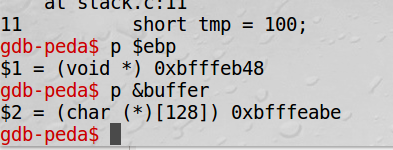
\includegraphics[scale=0.7]{2/4.png}\\\\
Here is the completed exploit code function:\\\\
\pagebreak
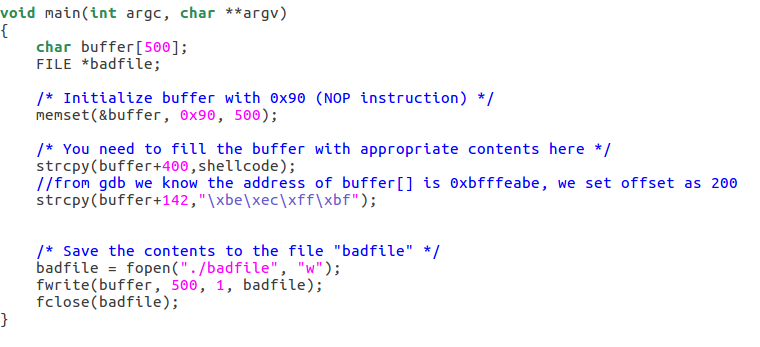
\includegraphics[scale=0.7]{2/5.png}\\
Now we compile and run it. This generated the contents for \verb+badfile+. I then ran the vulnerable program stack and got a root shell:\\\\
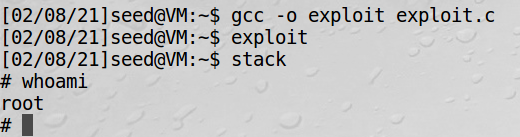
\includegraphics[scale=0.7]{2/6.png}\\\\
With the effective user id as root:\\\\
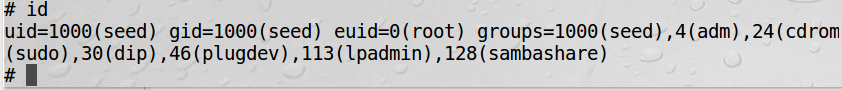
\includegraphics[scale=0.7]{2/7.png}\\
\subsection{Task 5: Defeating dash’s Countermeasure}
I first changed the \verb+/bin/sh+ symbolic link, so it points back to \verb+/bin/dash+ and activate the UID comparing:\\\\
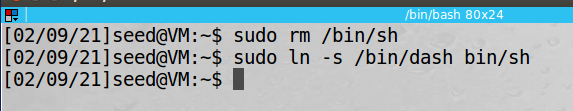
\includegraphics[scale=0.7]{2/8.png}\\\\
I commented the \verb+setuid(0);+ and ran the \verb+dash_shell_test+ program. It launches a bash shell without root privilege despite being a root-owned program.\\\\
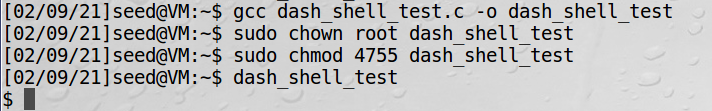
\includegraphics[scale=0.7]{2/9.png}\\\\
After we set the user id as root, the shell launched has root privilege.\\\\
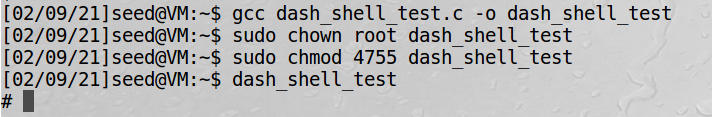
\includegraphics[scale=0.7]{2/10.png}\\\\
Next, I added the assembly code that calls \verb+setuid()+ to the shellcode and do another buffer overflow attack. I can get a root shell again despite the protection of \verb+/bin/sh+.\\\\
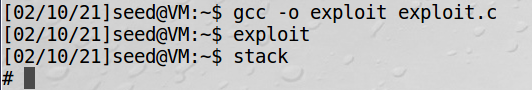
\includegraphics[scale=0.7]{2/12.png}
\subsection{Task 6: Defeating Address Randomization}
I turned on ASLR, and without doubt the attack did not work. It was because the address of the stack components are now randomized and the address in the shellcode is not the accurate one anymore.\\\\
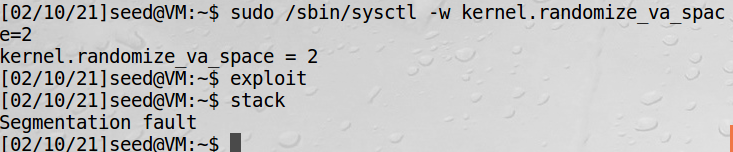
\includegraphics[scale=0.7]{2/13.png}\\\\
However with bruteforce attack we managed to defeat ASLR. By running the script provided, I obtained the root shell in 10.5 minutes. The attack succeeded.\\\\
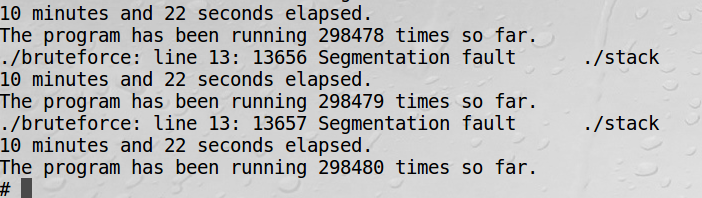
\includegraphics[scale=0.7]{2/14.png}
\subsection{Task 7: Turn on the StackGuard Protection}
By turning on the StackGuard protection, the system detects a change of the canary value and stopped the program from continuing. The attack failed despite the fact that ASLR was off.\\\\
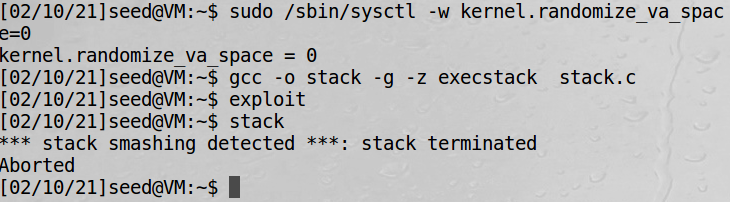
\includegraphics[scale=0.7]{2/15.png}
\subsection{Task 8: Turn on the Non-executable Stack Protection}
I turned on the NX stack protection with StackGuard off and ASLR off. I did not get a shell but there was segmentation fault error. There is still buffer overflow, but since my shellcode landed on a stack frame that is marked as NX, it was impossible to run. However the system is not safe as I could launch a return-to-libc attack instead.\\\\
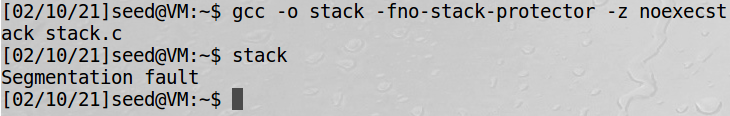
\includegraphics[scale=0.7]{2/16.png}\\
\pagebreak
\section{Format String Vulnerability}
\subsection{Task 9: Understanding the Layout of the Stack}
\subsubsection{Question 1-2}
Firstly I compiled the vulnerable program. There is a warning for the security issue but we ignore it.\\\\
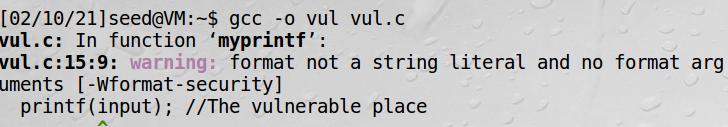
\includegraphics[scale=0.7]{3/1.png}\\\\
It runs smoothly if we simply input a short string with alphabets. It returns the string we typed. Note that the target address is \verb+0xbfffecd4+, which is the address of \verb+var+. Therefore the address of \verb+input+ would be \verb+0xbfffecd4+ + 4 = \verb+0xbfffecd8+.\\\\
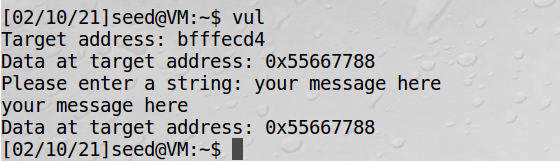
\includegraphics[scale=0.7]{3/2.png}\\\\
From the beginning of the format string, we used 5 \verb+%x+ to reach the beginning of \verb+var+. Therefore the address of the format string = \verb+0xbfffecd4+ - 20 = \verb+0xbfffecb4+.\\\\
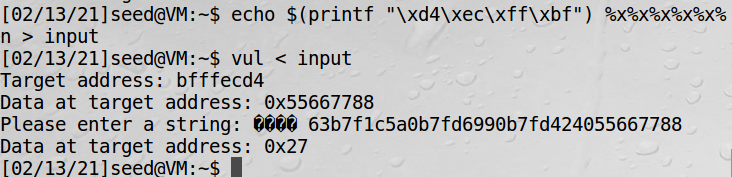
\includegraphics[scale=0.7]{3/3.png}
\subsection{Task 10: Crash the Program}
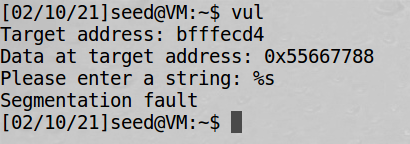
\includegraphics[scale=0.7]{3/7.png}
\subsection{Task 11: Print Out Data on the Stack}
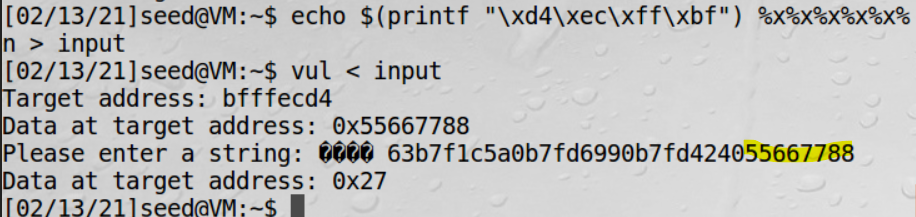
\includegraphics[scale=0.6]{3/13.png}
\subsection{Task 12: Change the Program’s Data in the Memory}
\subsubsection{Task 12.A: Change the value to a different value}
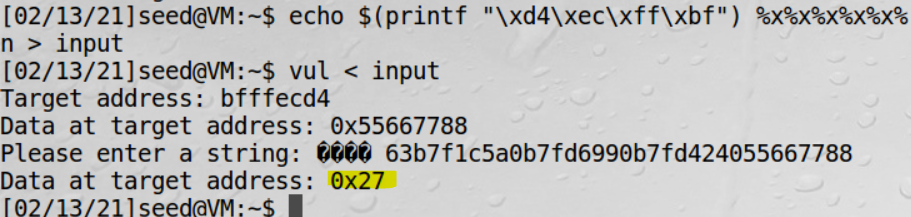
\includegraphics[scale=0.6]{3/14.png}
\subsubsection{Task 12.B: Change the value to 0x11221122}
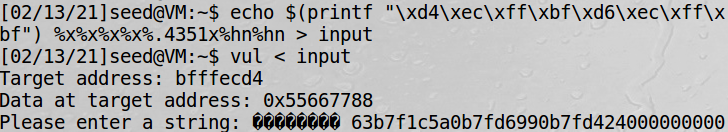
\includegraphics[scale=0.8]{3/9.png}\\\\
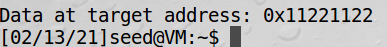
\includegraphics[scale=0.9]{3/10.png}
\subsubsection{Task 12.C: Change the value to 0x87654321}
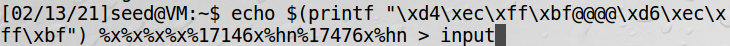
\includegraphics[scale=0.8]{3/11.png}\\\\
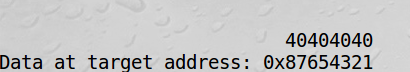
\includegraphics[scale=0.9]{3/12.png}

\end{document}